\documentclass[10pt]{beamer}
% \documentclass[handout,10pt]{beamer}
\usepackage{my_style}
%%%%%%%%%%%%%%%%%%%%%%%%%%%%%%%%%%%%%%%%%%%%%%%%%%%%%%%%%%%%%%%%%%%%%%%%

\title[Math/CS 375]{Lecture 04 - B}
\subtitle{\S 3.2  Newton’s Method}

\begin{document}
% -------------------------------------------------
\begin{frame}
  \titlepage
\end{frame}
% -------------------------------------------------
\begin{frame}{Goals}
We will answer these questions:\\[3mm]
\begin{itemize}
    \item How is Newton's method derived? 
    \item How fast does Newton's method converge?
    \item What are some drawbacks to Newton's method?
\end{itemize}
\end{frame}
%%%%%%%%%%%%%%%%%%%%%%%%%%%%%%%%%%%%%%%%%%%%%%%%%%%%%%%%%%%%%%%%%%%%%%%%
\sectionframe{Linearization}
%%%%%%%%%%%%%%%%%%%%%%%%%%%%%%%%%%%%%%%%%%%%%%%%%%%%%%%%%%%%%%%%%%%%%%%%

\begin{frame}{Linearization of a Function}

    \vspace{0.3cm}
    {\define{Linearization}{
    The \textbf{linearization} of a function \( f(x) \) at \( x = a \) is the equation of the tangent line to \( f(x) \) at that point:
    \[
    L(x) = f(a) + f'(a)(x - a)
    \]
    }}
    
    \vspace{0.5cm}
    \textbf{Steps to Find the Linearization:}
    \begin{enumerate}
        \item Evaluate the function at \( x = a \): \quad \( f(a) \)
        \item Compute the derivative \( f'(x) \) and evaluate it at \( x = a \): \quad \( f'(a) \)
        \item Substitute these values into the formula for the linearization:
        \[
        L(x) = f(a) + f'(a)(x - a)
        \]
    \end{enumerate}
\end{frame}
%%%%%%%%%%%%%%%%%%%%%%%%%%%%%%%%%%%%%%%%%%%%%%%%%%%%%%%%%%%%%%%%%%%%%%%%
\begin{frame}{Linearization}{Example}
    \begin{example}
    Find the linearization of \( f(x) = \cos(x)-x \) at \( x = \frac{\pi}{2} \).
    \end{example}
    \begin{align*}
        L(x) &= f(a) + f'(a)(x - a)\\
         &= f\left(\frac{\pi}{2}\right) + f'\left(\frac{\pi}{2}\right)(x-\frac{\pi}{2})\\
         &= \left(-\frac{\pi}{2}\right) +\left(-\sin\left(\frac{\pi}{2}\right)-1\right)(x-\frac{\pi}{2})\\
         &= -\frac{\pi}{2}- 2(x-\frac{\pi}{2})\\
         &= - 2x + \frac{\pi}{2}\\
    \end{align*}
Therefore, near $x=\frac{\pi}{2}$,
\[
\cos(x)-x \approx -2x+\frac{\pi}{2}.
\]
\end{frame}
%%%%%%%%%%%%%%%%%%%%%%%%%%%%%%%%%%%%%%%%%%%%%%%%%%%%%%%%%%%%%%%%%%%%%%%%
% \begin{frame}{Linearization}{Visualizing}
%     \begin{center}
%     \begin{tikzpicture}[scale=1.1]
%         \begin{axis}[
%             axis lines = middle,
%             xlabel = $x$, ylabel = $y$,
%             xmin = -0.2, xmax = 3.1,
%             ymin = -4, ymax = 2,
%             width=8cm,
%             height=6cm,
%             grid=both,
%             legend style={at={(1,1)},anchor=north}
%         ]
%         % Plot the function sin(x)
%         \addplot[blue, thick, domain=-0.2:3.1, samples=50] {cos(deg(x))-x};
%         \addlegendentry{$f(x) = \cos x - x$}
        
%         % Plot the linearization L(x) = x
%         \addplot[red, thick, domain=-0.2:3.1, samples=50] {-2*x+pi/2};
%         \addlegendentry{$L(x) = -2x + \frac{\pi}{2}$}
%         \end{axis}
%     \end{tikzpicture}
%     \end{center}

%     \vspace{0.3cm}
%     \question{
%         Can we use $L(x)$ to estimate the root of $f(x)$?
%     }
% \end{frame}
% %%%%%%%%%%%%%%%%%%%%%%%%%%%%%%%%%%%%%%%%%%%%%%%%%%%%%%%%%%%%%%%%%%%%%%%%
% \begin{frame}{Linearization}{Visualizing}
%     \begin{center}
%     \begin{tikzpicture}[scale=0.7]
%         \begin{axis}[
%             axis lines = middle,
%             xlabel = $x$, ylabel = $y$,
%             xmin = -0.2, xmax = 3.1,
%             ymin = -4, ymax = 2,
%             width=8cm,
%             height=6cm,
%             grid=both,
%             legend style={at={(1,1)},anchor=north}
%         ]
%         % Plot the function sin(x)
%         \addplot[blue, thick, domain=-0.2:3.1, samples=50] {cos(deg(x))-x};
%         \addlegendentry{$f(x) = \cos x - x$}
        
%         % Plot the linearization L(x) = x
%         \addplot[red, thick, domain=-0.2:3.1, samples=50] {-2*x+pi/2};
%         \addlegendentry{$L(x) = -2x + \frac{\pi}{2}$}
%         \end{axis}
%     \end{tikzpicture}
%     \end{center}
%     \begin{itemize}
%         \item Set $L(x)=0$ and solve for $x$
%         \item $L(x) = -2x +\pi/2=0 \implies x = \pi/4$
%         \item So the answer to $cos(x)-x=0$ is roughly $\pi/4\approx 0.78$
%         \item True answer is about $0.73$
%     \end{itemize}

% \end{frame}

%%%%%%%%%%%%%%%%%%%%%%%%%%%%%%%%%%%%%%%%%%%%%%%%%%%%%%%%%%%%%%%%%%%%%%%%
\begin{frame}{Can a Linearization Find a Root?}

\begin{center}
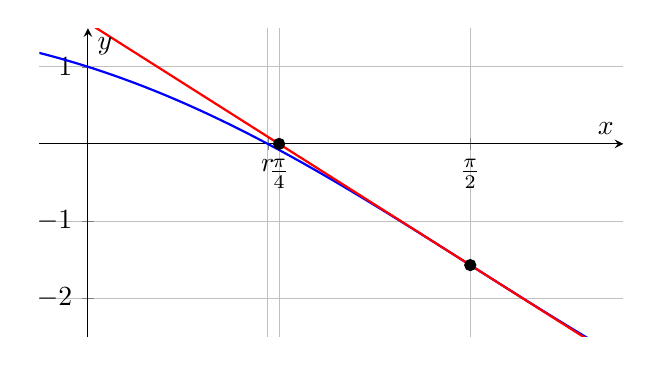
\begin{tikzpicture}
\begin{axis}[
    axis lines=middle,
    xlabel={$x$},
    ylabel={$y$},
    xmin=-0.2, xmax=2.2,
    ymin=-2.5, ymax=1.5,
    width=9cm,
    height=5.5cm,
    grid=both,
    xtick={0.739085,0.785398,1.5708},
    xticklabels={$r$,$\frac{\pi}{4}$,$\frac{\pi}{2}$},
]

\addplot[blue, thick, domain=-0.2:2.2, samples=100]
    {cos(deg(x))-x};

\addplot[red, thick, domain=-0.2:2.2]
    {-2*x+pi/2};

\addplot[only marks, mark=*]
    coordinates {(1.5708,-1.5708)};

\onslide<2->{
\addplot[only marks, mark=*]
    coordinates {(0.785398,0)};
}

\end{axis}
\end{tikzpicture}
\end{center}

\onslide<1>{
\question{
Can we use the easier function $L(x)$ to estimate
the root of $f(x)$?
}
}

\onslide<2->{
\[
L(x)=0
\quad\Longrightarrow\quad
-2x+\frac{\pi}{2}=0
\quad\Longrightarrow\quad
x=\frac{\pi}{4}\approx0.785.
\]
\begin{center}
    \small 
    (True answer is about $0.73$)
\end{center}
}
\end{frame}


\begin{frame}{Linearization}
\begin{block}{Nonlinear Problem}
Solving 
$$\cos(x)-x=0$$
is \textit{impossible}.
\end{block}

\begin{block}{Linearized Problem}
Approximate the function with a straight line
$$\cos(x)-x\approx -2x+\frac{\pi}{2}$$
Solving 
$$
-2x+\frac{\pi}{2}=0
$$
is \textit{trivial}.
\end{block}

\keyidea{Linearization can help us approximate the root of nonlinear functions.}
\end{frame}

%%%%%%%%%%%%%%%%%%%%%%%%%%%%%%%%%%%%%%%%%%%%%%%%%%%%%%%%%%%%%%%%%%%%%%%%
\sectionframe{Newton's Method}
%%%%%%%%%%%%%%%%%%%%%%%%%%%%%%%%%%%%%%%%%%%%%%%%%%%%%%%%%%%%%%%%%%%%%%%%


\begin{frame}{Do It Again}
\begin{itemize}
   
\item Start with an initial guess $x_0$ and linearize
$$ f(x) \approx L_0(x)$$
\item Solve $L_0(x)=0$ to get $x_1$

\[
x_0
\quad\longrightarrow\quad
x_1
\]

\vfill



\item<2-> Then we can use $x_1$ as the center of a new linearization $L_1(x)$ and get $x_2$
\[
x_0
\quad\longrightarrow\quad
x_1
\quad\longrightarrow\quad
x_2
\]


\vfill

\item<3-> We can do this an infinite number of times
\[
x_0
\quad\longrightarrow\quad
x_1
\quad\longrightarrow\quad
x_2
\quad\longrightarrow\quad x_3 \quad\cdots
\]

\onslide<4->{
\keyidea{
We can repeatedly use linearization to get closer to the true root.
}
}

\end{itemize}
\end{frame}

%%%%%%%%%%%%%%%%%%%%%%%%%%%%%%%%%%%%%%%%%%%%%%%%%%%%%%%%%%%%%%%%%%%%%%%%
%%%%%%%%%%%%%%%%%%%%%%%%%%%%%%%%%%%%%%%%%%%%%%%%%%%%%%%%%%%%%%%%%%%%%%%%
\begin{frame}{Visual}

\begin{center}
\begin{tikzpicture}
\begin{axis}[
    width=10cm,
    height=6cm,
    axis lines=middle,
    xmin=0, xmax=4.2,
    ymin=-1.2, ymax=4,
    xlabel={$x$},
    ylabel={$y$},
    xtick=\empty,
    ytick=\empty,
    samples=100,
    clip=false
]

% ------------------------------------------------
% Function: f(x) = 0.7(x-1)^2 - 0.8
% ------------------------------------------------
\addplot[
    blue,
    thick,
    domain=0.4:3.7
]
{0.7*(x-1)^2 - 0.8};

\node[blue] at (axis cs:1,-1.2) {$f(x)$};

% ================================================================
% FIRST ITERATION
% ================================================================
\only<1>{

% x_0
\addplot[
    only marks,
    mark=*,
    mark size=2pt
]
coordinates {(3,0)};

\node[below] at (axis cs:3,0) {$x_0$};

% f(x_0)
\addplot[
    dashed
]
coordinates {(3,0) (3,2)};

\addplot[
    only marks,
    mark=*,
    mark size=2pt
]
coordinates {(3,2)};

% Tangent line at x_0
% f'(x) = 1.4(x-1), so f'(3)=2.8
\addplot[
    red,
    thick,
    domain=1.8:3.7
]
{2.8*(x-3)+2};

\node[red, above,left] at (axis cs:3.35,3.0)
    {$L_0(x)$};

% x_1 = tangent-line root
\addplot[
    only marks,
    red,
    mark=*,
    mark size=2pt
]
coordinates {(2.2857,0)};

\node[red, below] at (axis cs:2.2857,0)
    {$x_1$};

}

% ================================================================
% SECOND ITERATION
% ================================================================
\only<2>{
% x_1
\addplot[
    only marks,
    mark=*,
    mark size=2pt
]
coordinates {(2.2857,0)};

\node[below] at (axis cs:2.2857,0) {$x_1$};

% f(x_1)
\addplot[
    dashed
]
coordinates {(2.2857,0) (2.2857,0.3571)};

\addplot[
    only marks,
    mark=*,
    mark size=2pt
]
coordinates {(2.2857,0.3571)};

% Tangent line at x_1
% f'(2.2857) = 1.8
\addplot[
    red,
    thick,
    domain=1.7:3.1
]
{1.8*(x-2.2857)+0.3571};

\node[red, above] at (axis cs:2.8,1.35)
    {$L_1(x)$};

% x_2 = tangent-line root
\addplot[
    only marks,
    red,
    mark=*,
    mark size=2pt
]
coordinates {(2.0873,0)};

\node[red, below] at (axis cs:2.0873,0)
    {$x_2$};

}
\end{axis}
\end{tikzpicture}
\end{center}

% \onslide<1>{
% \[
% x_1=\text{root of the linearization at }x_0
% \]
% }

% \onslide<2>{
% \[
% x_2=\text{root of the linearization at }x_1
% \]
% }

\begin{itemize}
    \item<1-> Linearize around $x_0$ and solve $L_0(x_1)=0$ 
    \item<2-> Linearize around $x_1$ and solve $L_1(x_2)=0$
\end{itemize}
\end{frame}

%%%%%%%%%%%%%%%%%%%%%%%%%%%%%%%%%%%%%%%%%%%%%%%%%%%%%%%%%%%%%%%%%%%%%%%%
\begin{frame}{Formula}

\begin{itemize}
    \item  Suppose our current approximation is $x_k$.

\vfill

\item Linearize $f$ around $x_k$ is
\[
f(x)\approx L(x)=
f(x_k)+f'(x_k)(x-x_k).
\]

\vfill

\item We choose $x_{k+1}$ to be the root of this tangent line:
\[
L(x_{k+1})=0.
\]


\item<2-> Therefore,
\[
0
=
f(x_k)+f'(x_k)(x_{k+1}-x_k).
\]

\vfill

\onslide<3->{
Solving for $x_{k+1}$ gives us the update formula 
\[
\boxed{
x_{k+1}
=
x_k-\frac{f(x_k)}{f'(x_k)}.
}
\]
}
\end{itemize}

\end{frame}

%%%%%%%%%%%%%%%%%%%%%%%%%%%%%%%%%%%%%%%%%%%%%%%%%%%%%%%%%%%%%%%%%%%%%%%%
\begin{frame}[fragile]{Newton's Method}


    \begin{block}{Formula}
    Start with an initial guess $x_0$ then iterate using the recurrence formula:
    \begin{equation*}
            x_{k+1} = x_k - \frac{f(x_k)}{f'(x_k)}.
\end{equation*}

    \end{block}

{
\method{Newton's Method}{$f(x)$, $f'(x)$, initial guess $x_0$}{approximate solution to $f(x)=0$}{
Leverage function's derivative to converge quickly.
}
}


\medskip
{
\begin{block}{Why ``Newton's Method''?}
Newton developed an early version of the method in the 1600s.
Raphson later simplified the iteration into a form closer to
the one used today.  For this reason, it is also called the
\textbf{Newton-Raphson method}.
\end{block}
}

\end{frame}
%%%%%%%%%%%%%%%%%%%%%%%%%%%%%%%%%%%%%%%%%%%%%%%%%%%%%%%%%%%%%%%%%%%%%%%%
\begin{frame}{Newton By Hand}
\begin{example}
Write a Newton recurrence formula to solve the equation
\begin{equation*}
    x = x^{1/3} + 2 
\end{equation*}
starting with $x_0 = 3$.
\end{example}

\begin{itemize}
    \item First, rewrite the equation in the form $f(x)=0$: 
        \begin{align*}
                x &= x^{1/3} + 2\\ 
                x - x^{1/3} - 2 &=0  
        \end{align*}
\item Next, find the derivative 
\begin{equation*}
    f'(x) = 1 - \frac{1}{3}x^{-2/3}
\end{equation*}
\item Substitute into the recurrence formula 
\begin{equation*}
    x_{k+1} = x_k - \frac{x_k - x_k^{1/3} - 2}{1 - \frac{1}{3}x_k^{-2/3}}
\end{equation*}
\end{itemize}
\end{frame}

%%%%%%%%%%%%%%%%%%%%%%%%%%%%%%%%%%%%%%%%%%%%%%%%%%%%%%%%%%%%%%%%%%%%%%%%
\begin{frame}{Numerical Test}

\begin{equation*}
    x_{k+1} = x_k - \frac{x_k - x_k^{1/3} - 2}{1 - \frac{1}{3}x_k^{-2/3}}
\end{equation*}

\begin{center}
  \small
    \renewcommand{\arraystretch}{1.3}
    \begin{tabular}{cccc}
    $k$ &    $x_k$     & $f'(x_k)$  &   $f(x)$                   \\ \hline
     0  &  3           & 0.83975005 & -0.44224957                \\
     1  &  3.52664429  & 0.85612976 &  0.00450679                \\
     2  &  3.52138015  & 0.85598641 &  $3.771\times 10^{-7}$   \\
     3  &  3.52137971  & 0.85598640 &  $2.664\times 10^{-15}$ \\
     4  &  3.52137971  & 0.85598640 &  0.0                       \\
    \end{tabular}
\end{center}

\begin{itemize}
    \item Newton's method finishes in only \textbf{4 iterations} 
    \item Bisection requires around \textbf{50 iterations}
    \item Newton's method has a fast rate of convergence
\end{itemize}
\end{frame}

%%%%%%%%%%%%%%%%%%%%%%%%%%%%%%%%%%%%%%%%%%%%%%%%%%%%%%%%%%%%%%%%%%%%%
\sectionframe{Convergence Analysis}
%%%%%%%%%%%%%%%%%%%%%%%%%%%%%%%%%%%%%%%%%%%%%%%%%%%%%%%%%%%%%%%%%%%%%
\begin{frame}[shrink]{Convergence Theorem}

\begin{block}{Recall: Convergence Rate}
  Convergence of a method is said to be of order $r$ if there is a
constant $C>0$ 
\begin{equation*}
  \lim_{k\rightarrow \infty} \frac{|e_{k+1}|}{|e_k|^r} \leq C
\end{equation*}
\end{block}
\bigskip

\begin{theorem}
Suppose 
\begin{itemize}
    \item $f$ is sufficiently smooth near the root $x_*$
    \item The derivative at the root $f'(x_*) \ne 0$
    \item Initial guess $x_0$ is sufficiently close to $x_*$
\end{itemize}
Then Newton's Method converges with order $r=2$ (quadratic).

\end{theorem}


\end{frame}
%%%%%%%%%%%%%%%%%%%%%%%%%%%%%%%%%%%%%%%%%%%%%%%%%%%%%%%%%%%%%%%%%%%%%%%%
\begin{frame}{Proof}{Part 1}
\begin{itemize}
\item Suppose the true root of $f(x)$ is $x_*$. Then by Taylor's theorem: 
    \begin{equation*}
      f(x_{*}) = f(x_k) + (x_{*}-x_k)f'(x_k) + \frac{1}{2}(x_{*}-x_k)^2 f''(\xi) \equiv 0 
    \end{equation*}
\item Factor out $f'(x_k)$ to get
\begin{equation*}
   \frac{f(x_k)}{f'(x_k)} + x_{*}-x_k + (x_{*}-x_k)^2 \left(\frac{1}{2}\right) \frac{f''(\xi)}{f'(x_k)} = 0
\end{equation*}
\item Then
\begin{equation*}
  \left(\frac{f(x_k)}{f'(x_k)} -x_k\right)+ x_{*} + (x_{*}-x_k)^2 \left(\frac{1}{2}\right) \frac{f''(\xi)}{f'(x_k)} = 0
\end{equation*}
\begin{equation*}
  x_{*}-x_{k+1} + (x_{*}-x_k)^2 \left(\frac{1}{2}\right) \frac{f''(\xi)}{f'(x_k)} = 0
\end{equation*}
\item Factor out $(x_{*}-x_k)^2$ to get
\begin{equation*}
  \frac{x_{*}-x_{k+1}}{(x_{*}-x_k)^2}  = -\left(\frac{1}{2}\right) \frac{f''(\xi)}{f'(x_k)}
\end{equation*}
\end{itemize}
\end{frame}

%%%%%%%%%%%%%%%%%%%%%%%%%%%%%%%%%%%%%%%%%%%%%%%%%%%%%%%%%%%%%%%%%%%%%%%%
\begin{frame}{Proof}{Part 2}

\begin{itemize}
\item If we define error to be $e_k = x_* - x_k$ then in absolute value 
\begin{equation*}
  \frac{\left|x_{*}-x_{k+1}\right|}{\left|x_{*}-x_k\right|^2}  = 
  \frac{ | e_{k+1} | }{ |e_k|^2} =  \left(\frac{1}{2}\right) \left|\frac{f''(\xi)}{f'(x_k)}\right|
\end{equation*}
\item We assumed $f$ to be smooth and $f'(x_*) \ne 0$ so 
$$\left|\frac{f''(\xi)}{f'(x_k)}\right| < C$$

\item We have shown that 
    $$\frac{ | e_{k+1} | }{ |e_k|^2} \le  \left(\frac{C}{2}\right)$$ 
\end{itemize}

\keyidea{
    Equation $|e_{k+1}| = C|e_k|^2 $ means that errors decreases \textbf{quadratically} ($r=2$). This is an entire order faster than bisection ($r=1$).
}

\end{frame}

\begin{frame}{Quadratic Convergence}

\question{How fast is quadratic convergence?}

\begin{itemize}
    \item Suppose your starting error is 
    $$E_0=10^{-2}$$

    \item<2-> After one iteration
    $$
    E_1 \approx E_0^2 = 10^{-4}
    $$
    \item<3-> Second iteration
    $$
    E_2 \approx E_1^2 = 10^{-8}
    $$
    \item<4-> And third 
    $$
    E_3 \approx E_2^2 = 10^{-16} \approx \epsilon_m
    $$
    \vfill 
    \item<4> Quadratic convergence is \textit{very} fast
\end{itemize}
\end{frame}

%%%%%%%%%%%%%%%%%%%%%%%%%%%%%%%%%%%%%%%%%%%%%%%%%%%%%%%%%%%%%%%%%%%
\sectionframe{Some Issues}
%%%%%%%%%%%%%%%%%%%%%%%%%%%%%%%%%%%%%%%%%%%%%%%%%%%%%%%%%%%%%%%%%%%
\begin{frame}{Issue 1: Divergence}

\begin{center}
	\pgfimage[height=3cm]{./figs/NewtonFails}
\end{center}

\begin{itemize}
    \item If \( f'(x_1) \approx 0 \), then the update \( x_2 \) may jump very far away
    \item In this case, Newton's method may \textbf{diverge} ($|x_k| \rightarrow \infty$)
    \item If \( f'(x_k) =0 \) then we have division by zero in 
    $$x_{k+1} = x_k - \frac{f(x_k)}{f'(x_k)}$$
\end{itemize}
\end{frame}
%%%%%%%%%%%%%%%%%%%%%%%%%%%%%%%%%%%%%%%%%%%%%%%%%%%%%%%%%%%%%%%%%%%
\begin{frame}{Issue 2: Infinite Cycle}
    Consider finding the root of the following function with Newton's method
        \[
        f(x) = x^3 - 2x + 2.
        \]
\begin{itemize}
    \item The iteration becomes
        \[
        x_{k+1} = x_k - \frac{x_k^3 - 2x_k + 2}{3x_k^2 - 2}.
        \]
    \item Starting with \( x_0 = 0 \):
\begin{center}
  \small
  \renewcommand{\arraystretch}{1.3}
  \begin{tabular}{cccc}
    \(k\) & \(x_k\) & \(f'(x_k)\) & \(f(x_k)\) \\ \hline
     0   &  0      & -2         & 2         \\
     1   & -1      & 1          & 3         \\
     2   &  1      & 1          & 1         \\
     3   & -1      & 1          & 3         \\
     4   &  1      & 1          & 1         
  \end{tabular}
\end{center}
    \item Newton's method is stuck in an infinite two-stage cycle
\end{itemize}
\end{frame}
%%%%%%%%%%%%%%%%%%%%%%%%%%%%%%
\begin{frame}{Issue 3: Slow Convergence}

{\define{Multiple Zeros}{
\begin{itemize}
    \item  A function has a \textbf{double zero} at \(x_*\) if \(f(x_*) = 0\) and \(f'(x_*) = 0\).
    
    \item More generally, a function has a root of \textbf{multiplicity} \( m \) if 
    \[
    f^{(k)}(x_*) = 0, \quad 0 \leq k < m, \quad \text{and} \quad f^{(m)}(x_*) \neq 0.
    \]
\end{itemize}
}}

\begin{itemize}
    \item For example, \( p(x) = x^2 - 2x + 1 = (x-1)^2 \) has a double zero at \( x = 1 \)
    \begin{itemize}
        \item $p(1) = 0$
        \item $p'(1)=2-2 = 0$
        \item $p''(1)= 2 \ne 0$
    \end{itemize}
    \item Newton's method exhibits slow convergence when the root has multiple zeros

{\begin{theorem}
    If $f(x)$ has a root at $x_*$ of multiplicity $m\ge 2$ then Newton's method converges to $x_*$ at a \textbf{linear rate}. 
\end{theorem}}
\end{itemize}
\end{frame}
% %%%%%%%%%%%%%%%%%%%%%%%%%%%%%%
% \begin{frame}{Slow Convergence Proof}{Part 1}

% Taylor series expansion of a function \( f(x) \) about \( x = x^* \):
% \[
% f(x) = f(x^*) + f'(x^*)(x-x^*) + \frac{f''(x^*)}{2}(x-x^*)^2 + \cdots
% \]
% Since \( x^* \) is a double zero $(f(x^*)=0 \quad \text{and} \quad f'(x^*)=0)$, we get the approximation
% \[
% \boxed{
% f(x) \approx \frac{f''(x^*)}{2}(x - x^*)^2.
% }
% \]

% Similarly, for the derivative \( f'(x) \), its Taylor expansion about \( x=x^* \) is:
% \[
% f'(x) = f'(x^*) + f''(x^*)(x-x^*) + \cdots,
% \]
% and since \( f'(x^*)=0 \), we obtain:
% \[
% \boxed{
% f'(x) \approx f''(x^*)(x - x^*).
% }
% \]
% \end{frame}

% %%%%%%%%%%%%%%%%%%%%%%%%%%%%%%

% \begin{frame}{Slow Convergence Proof}{Part 2}
% Substituting $x_k$ into our previous formulas yield:
% \[
% f(x_k) \approx \frac{f''(x^*)}{2}(x_k - x^*)^2, \quad 
% f'(x_k) \approx f''(x^*)(x_k - x^*).
% \]
% Substitute these into Newton's update:
% \[
% x_{k+1} = x_k - \frac{f(x_k)}{f'(x_k)}
% \approx x_k - \frac{\frac{f''(x^*)}{2}(x_k - x^*)^2}{f''(x^*)(x_k - x^*)}.
% \]
% Simplify the expression:
% \[
% x_{k+1} \approx x_k - \frac{1}{2}(x_k - x^*).
% \]
% Subtract \(x^*\) from both sides:
% \[
% x_{k+1} - x^* \approx \frac{1}{2}(x_k - x^*).
% \]
% \end{frame}

% %%%%%%%%%%%%%%%%%%%%%%%%%%%%%%
% \begin{frame}{Slow Convergence Proof}{Part 3}
% \begin{itemize}
%     \item The relation
%     \[
%     |x_{k+1} - x^*| \approx \frac{1}{2}|x_k - x^*|
%     \]
%     indicates that Newton's method converges \textbf{linearly} when \( f'(x^*) = 0 \).
% \end{itemize}
% \begin{block}{Key Idea}
% \begin{itemize}
%     \item When \( f'(x^*) \neq 0 \), Newton's method typically converges \textbf{quadratically}, meaning the error roughly squares at each iteration.
    
%     \item When \( f'(x^*) = 0 \), Newton's method slows down to \textbf{linear} convergence.
% \end{itemize}
% \end{block}
% \end{frame}
%-------------------------------------------------
\begin{frame}{Slow Convergence Proof}{Part 1}

\begin{enumerate}
\item[1.] \textbf{Taylor expansion of $f$}.  
      We assume that \(f\) has a double zero \(f(x_{*}) = f'(x_{*}) = 0\). Then
      \begin{align*}
          f(x) &= f(x^{*}) + f'(x^{*})(x-x^{*}) + \tfrac12 f''(x^{*})(x-x^{*})^{2}+\cdots\\
               &\Longrightarrow\\
          \,f(x) &\approx \tfrac12 f''(x^{*})(x-x^{*})^{2}
      \end{align*}
    

\item[2.] \textbf{Taylor expansion of $f'$}  
      Likewise, the Taylor expansion of $f'(x)$ yields
      \begin{align*}
          f'(x) &= f'(x_{*}) + f''(x_{*})(x-x_{*}) + \cdots\\
          &\Longrightarrow\\
          f'(x) &\approx f''(x_{*})(x-x_{*}) 
      \end{align*}
\end{enumerate}

\end{frame}

%-------------------------------------------------
\begin{frame}{Slow Convergence Proof}{Part 2}

\begin{enumerate}
\item[3.] \textbf{Approximate \(f\) and \(f'\) at the current iterate.}
      \[
        f(x_k)   \;\approx\; \tfrac12 f''(x_{*})(x_k-x_{*})^{2}, 
        \qquad
        f'(x_k)  \;\approx\; f''(x_{*})(x_k-x_{*}).
      \]

\item[4.] \textbf{Insert these into Newton’s update.}
      \[
      x_{k+1}=x_k-\frac{f(x_k)}{f'(x_k)}
      \;\approx\;
      x_k - \frac{\tfrac12 f''(x^{*})(x_k-x^{*})^{2}}
                  {f''(x^{*})(x_k-x^{*})}
      =
      x_k - \tfrac12(x_k-x^{*}).
      \]

\item[5.] \textbf{Subtract $x^*$ both sides.}
      \[
        x_{k+1}-x^{*} \;\approx\; \tfrac12\,(x_k-x^{*}).
      \]
\end{enumerate}

\end{frame}

%-------------------------------------------------
\begin{frame}{Slow Convergence Proof}{Part 3}

\begin{itemize}
\item[6.] \textbf{Absolute value both sides.} We finally obtain an approximate relation between the new error and current error
      \[
        |x_{k+1}-x^{*}| 
        \;\approx\;
        \frac12\,|x_k-x^{*}|.
      \]

\end{itemize}

\keyidea{
\begin{itemize}
  \item If \(f'(x^{*})\neq 0\) (simple root), Newton’s method is \textbf{quadratic}:  
        \( |e_{k+1}| \propto |e_k|^{2}. \)
  \item If \(f'(x^{*}) = 0\) (double zero), the rate drops to \textbf{linear}:  
        \( |e_{k+1}| \approx \tfrac12 |e_k|. \)
\end{itemize}
}

\end{frame}
%%%%%%%%%%%%%%%%%%%%%%%%%%%%%%
\begin{frame}{Fix}
\begin{itemize}
    \item All of the issues with Newton's Method can be fixed by using an adaptive step size 

    $$ x_{k+1} = x_k - \alpha_k \frac{f(x_k)}{f'(x_k)}$$

    \item Many several choices for $\alpha_k $
        \begin{itemize}
            \item $\alpha = 1/2$
            \item $\alpha = m $ (the multiplicity) 
            \item $\alpha = \textrm{argmin}_\alpha \left|f\left(x_k - \alpha \frac{f(x_k)}{f'(x_k)}\right) \right|$
        \end{itemize}
\end{itemize}
\keyidea{
Drawbacks to the Newton's include:
\begin{itemize}
    \item Sensitivity to small slopes
    \item Infinite cycles
    \item Slow convergence due to multiple zeros 
\end{itemize}
but these obstacles can be overcome with a small modification.
}
\end{frame}


%%%%%%%%%%%%%%%%%%%%%%%%%%%%%%
\sectionframe{Extra Topic: Fractals}
%%%%%%%%%%%%%%%%%%%%%%%%%%%%%%%%%%%%%%%%%%
\begin{frame}
\frametitle{Fractals: What?}
\begin{definition}{Fractal:}
A mathematical pattern (geometric object) that is reproducible at {\bf{any}}
level of magnification or reduction.
\end{definition}

\begin{definition}{Fractal:}
A term used by Benoit Mandelbrot to refer to geometric objects with
fractional dimensions rather than integer dimensions.  Also used "fractal"
to refer to shapes that are self-similar: they look the same at any zoom
level.
\end{definition}
\end{frame}
%%%%%%%%%%%%%%%%%%%%%%%%%%%%%%%%%%%%%%%%%%%%%%%%%%%%%%%%%%%%%%%%%%%%%%%%
%%%%%%%%%%%%%%%%%%%%%%%%%%%%%%%%%%%%%%%%%%%%%%%%%%%%%%%%%%%%%%%%%%%%%%%%
\begin{frame}
\frametitle{Fractals: Application}
Scientificly used to describe highly irregular objects
\begin{itemize}
  \item Fractal image compression
  \item Seismology
  \item Cosmology
  \item Life sciences:
    \begin{itemize}
      \item Clouds and fluid turbulence
      \item Trees
      \item Coastlines
    \end{itemize}
\end{itemize}
More interesting observations:
\begin{itemize}
   \item New music/New art (Jackson Pollock)
  \item Video games/graphics
  \item Chaos theory
  \item The Butterfly effect: small changes produces large effects
\end{itemize}
\end{frame}
%%%%%%%%%%%%%%%%%%%%%%%%%%%%%%%%%%%%%%%%%%%%%%%%%%%%%%%%%%%%%%%%%%%%%%%%
\begin{frame}
\frametitle{Fractals: Air Pressure}
\framesubtitle{Air channels between two glued pieces of acrylic}
\begin{center}
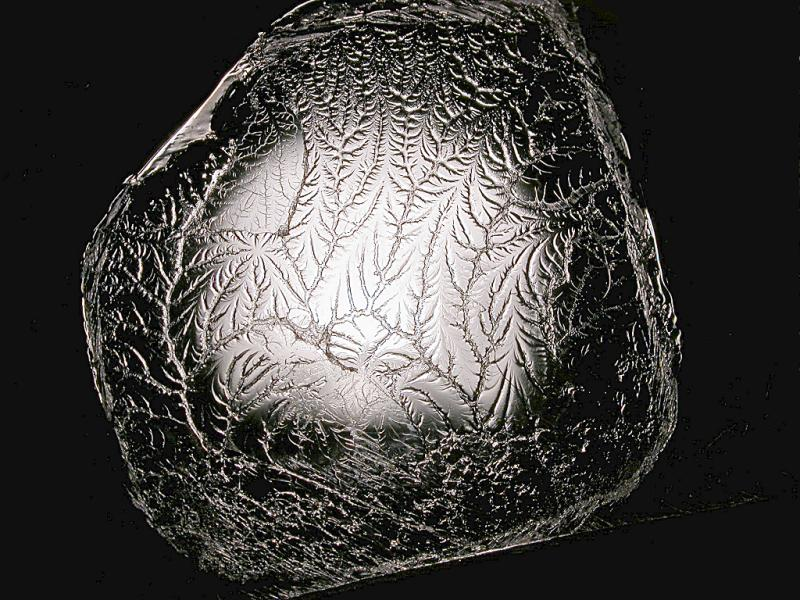
\includegraphics[height=0.9\textheight]{figs/fractal1}
\end{center}
\end{frame}
\begin{frame}
\frametitle{Fractals: high voltage dielectric breakdown}
\framesubtitle{Lichtenberg: Branching discharges decrease to hairlike then to
molecular}
\begin{center}
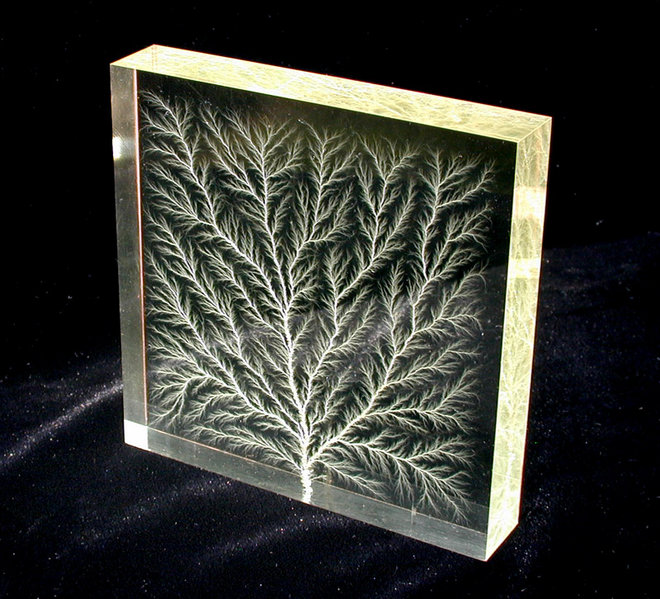
\includegraphics[height=0.9\textheight]{figs/fractal2}
\end{center}
\end{frame}
\begin{frame}
\frametitle{Fractals: Microwaving a CD}
\framesubtitle{Heat vaporizes the aluminum leaving fractal metallic islands}
\begin{center}
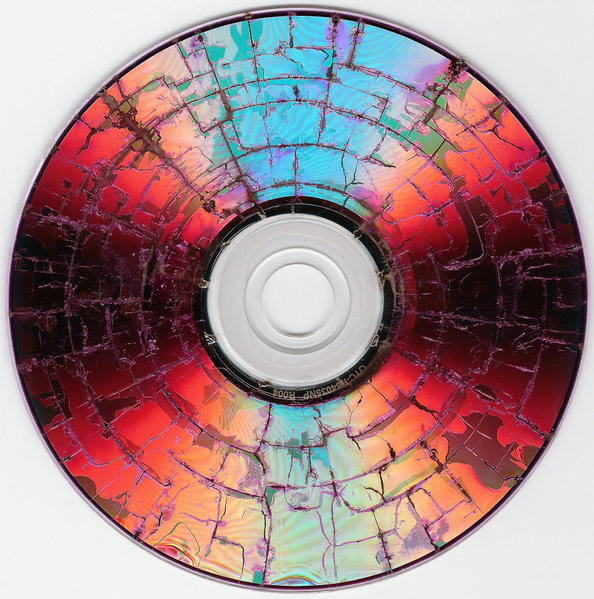
\includegraphics[height=0.9\textheight]{figs/fractal3}
\end{center}
\end{frame}
\begin{frame}
\frametitle{Fractals: Romanesco Broccoli}
\framesubtitle{Growth follows fractal pattern}
\begin{center}
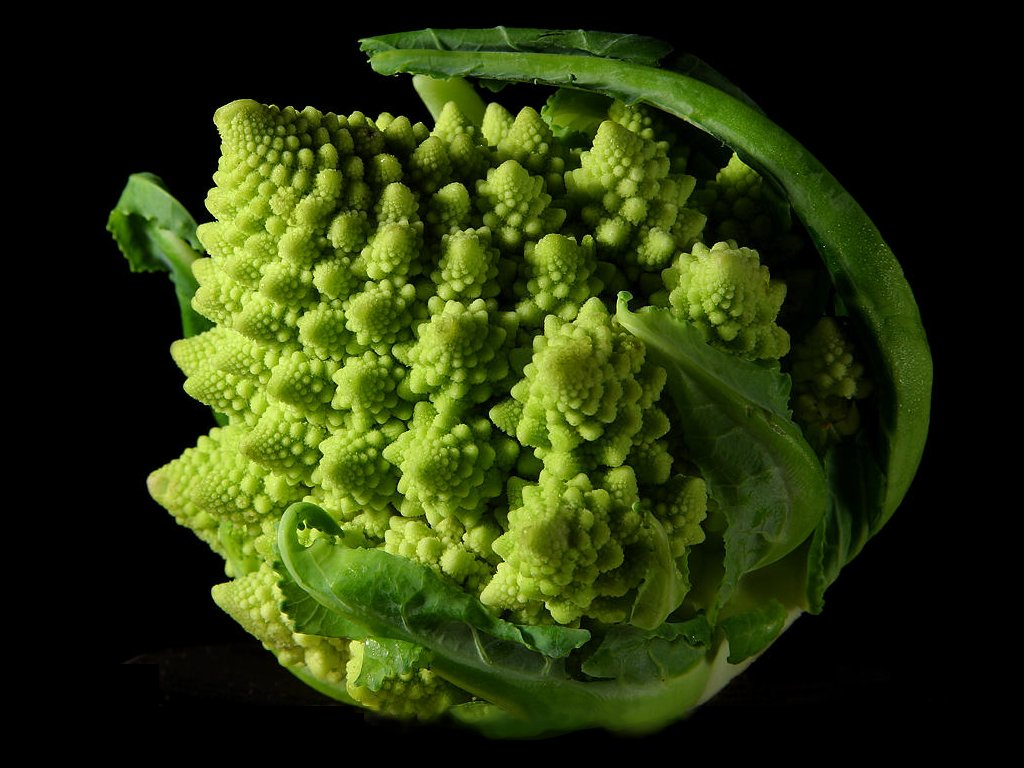
\includegraphics[height=0.9\textheight]{figs/fractal4}
\end{center}
\end{frame}

\begin{frame}
\frametitle{Fractals: Jupiter}
\framesubtitle{Atmosphere modeled with fractals}
\begin{center}
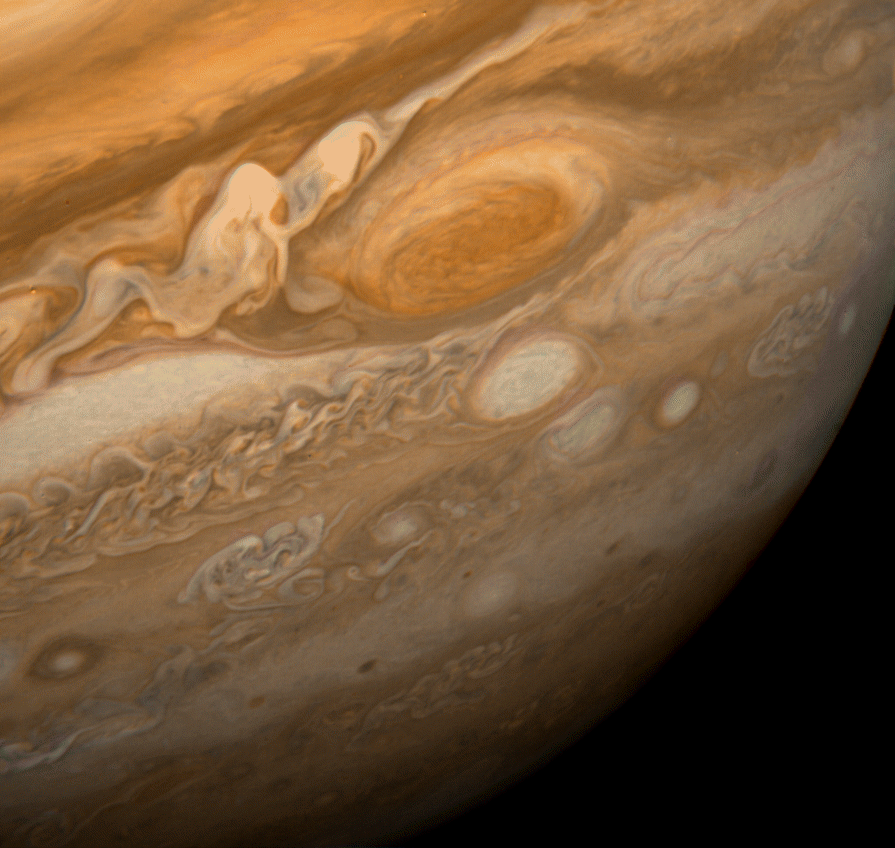
\includegraphics[height=0.9\textheight]{figs/fractal7}
\end{center}
\end{frame}
\begin{frame}
\frametitle{Fractals: Caves}
\framesubtitle{Stalactite/Stalagmite formation}
\begin{center}
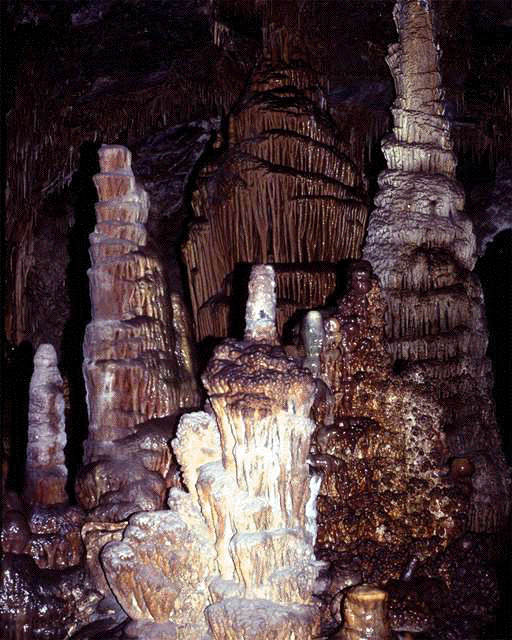
\includegraphics[height=0.9\textheight]{figs/fractal8}
\end{center}
\end{frame}
% \begin{frame}
% \frametitle{Fractals: Canyons}
% \framesubtitle{Erosion pattern}
% \begin{center}
% 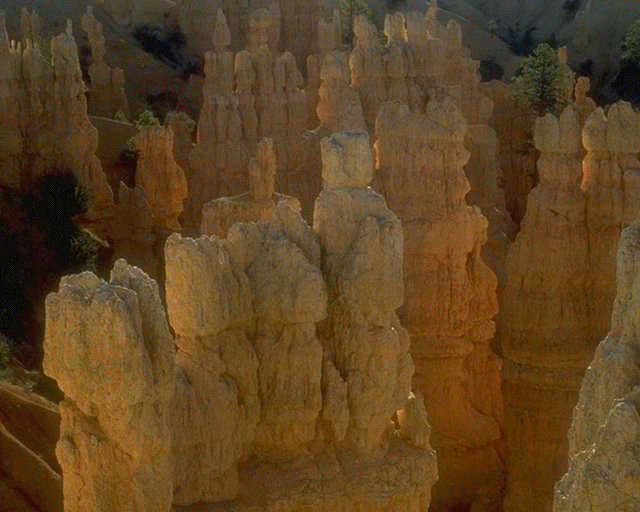
\includegraphics[scale=0.4]{figs/fractal9}
% \end{center}
% \end{frame}
% \begin{frame}
% \frametitle{Fractals: Clouds}
% \framesubtitle{Visualization}
% \begin{center}
% 
\includegraphics[height=0.9\textheight]{figs/fractal10}
% \end{center}
% \end{frame}
\begin{frame}
\frametitle{Fractals: Ferns}
\framesubtitle{Growth}
\begin{center}
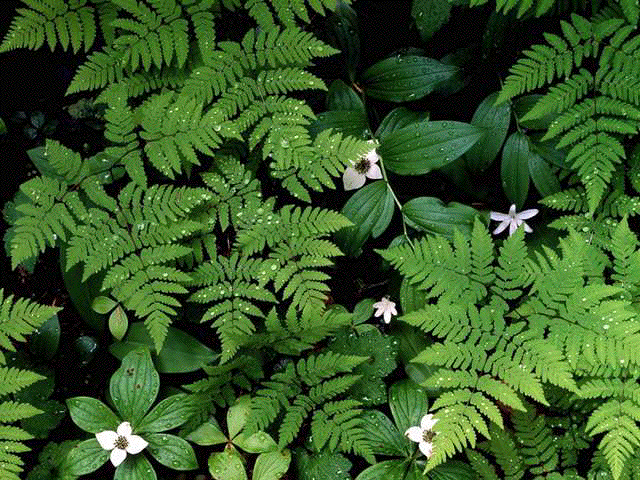
\includegraphics[height=0.9\textheight]{figs/fractal11}
\end{center}
\end{frame}
\begin{frame}
\frametitle{Fractals: Big Trees}
\framesubtitle{Growth}
\begin{center}
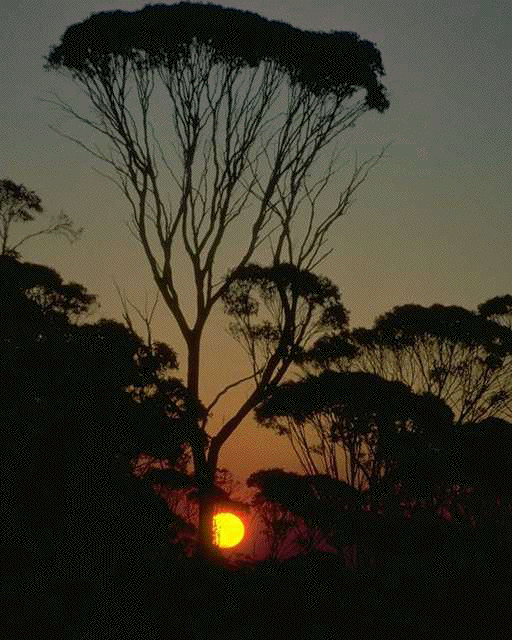
\includegraphics[height=0.9\textheight]{figs/fractal12}
\end{center}
\end{frame}

% \begin{frame}
% \frametitle{Fractals: lightning}
% \framesubtitle{Formation}
% \begin{center}
% 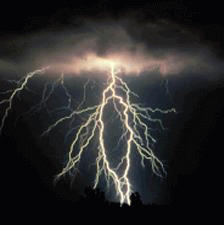
\includegraphics[height=0.9\textheight]{figs/fractal14}
% \end{center}
% \end{frame}
% \begin{frame}
% \frametitle{Fractals: cauliflower}
% \framesubtitle{Structure}
% \begin{center}
% 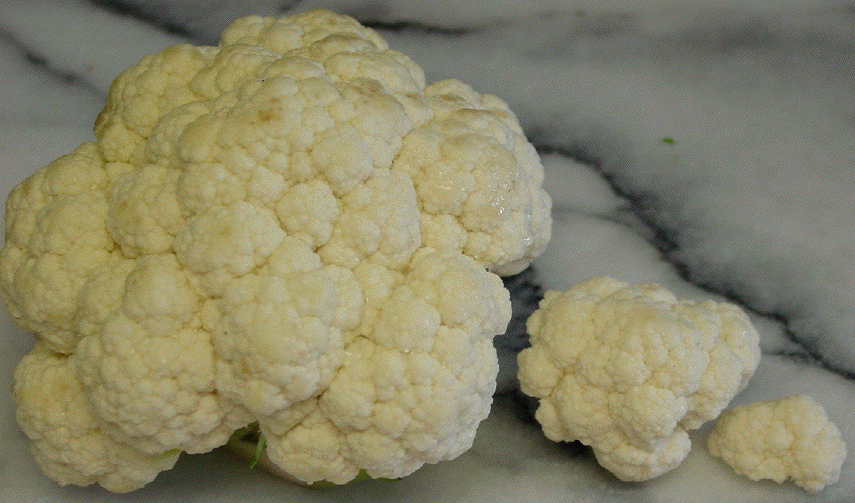
\includegraphics[height=0.9\textheight]{figs/fractal15}
% \end{center}
% \end{frame}
% \begin{frame}
% \frametitle{Fractals: mountain}
% \framesubtitle{Formation}
% \begin{center}
% 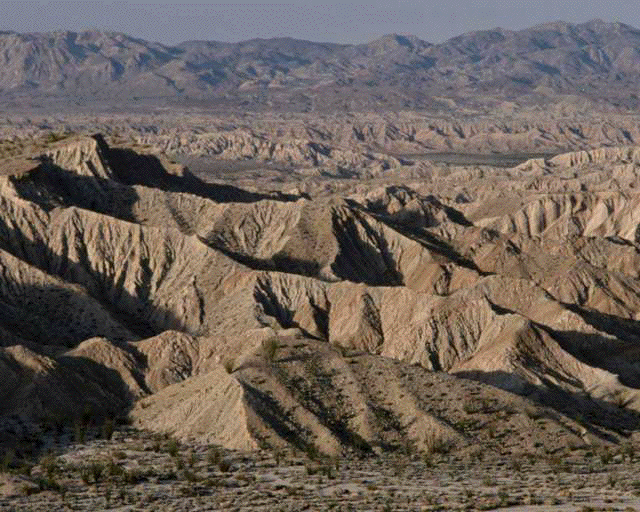
\includegraphics[height=0.9\textheight]{figs/fractal16}
% \end{center}
% \end{frame}
% \begin{frame}
% \frametitle{Fractals: mountain}
% \framesubtitle{Visualization}
% \begin{center}
% 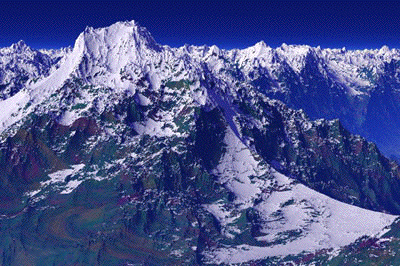
\includegraphics[height=0.9\textheight]{figs/fractal19}
% \end{center}
% \end{frame}
\begin{frame}
\frametitle{Fractals: Norwegian rivers}
\framesubtitle{Structure}
\begin{center}
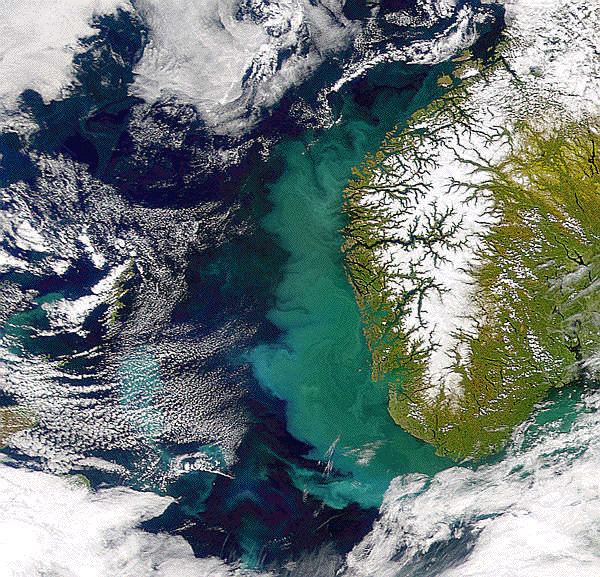
\includegraphics[height=0.9\textheight]{figs/fractal17}
\end{center}
\end{frame}
\begin{frame}
\frametitle{Fractals: waterfalls}
\framesubtitle{Pattern}
\begin{center}
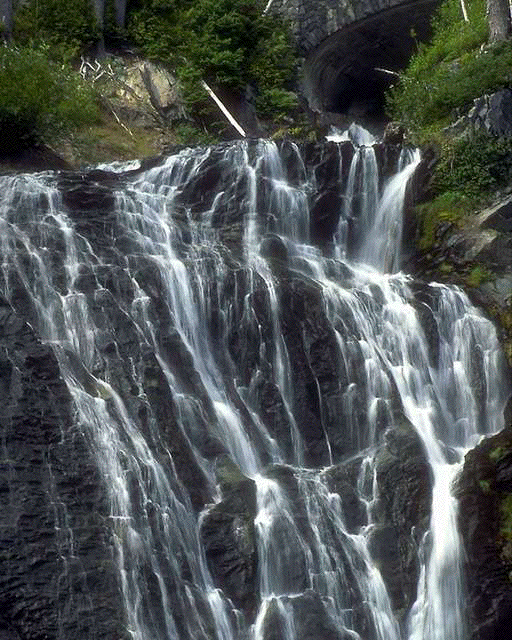
\includegraphics[height=0.9\textheight]{figs/fractal18}
\end{center}
\end{frame}
% \begin{frame}
% \frametitle{Fractals: coastlines}
% \framesubtitle{Structure}
% \begin{center}
% 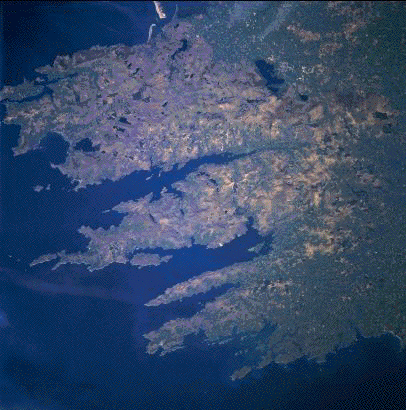
\includegraphics[height=0.9\textheight]{figs/fractal20}
% \end{center}
% \end{frame}
%%%%%%%%%%%%%%%%%%%%%%%%%%%%%%%%%%%%%%%%%%%%%%%%%%%%%%%%%%%%%%%%%%%%%%%%
\begin{frame}
\frametitle{Fractals: Math}
Recall Complex Numbers: $z \in \mathbb{C}$ means
\begin{equation*}
  z = x + i y,
\end{equation*}
where $i = \sqrt{-1}$
\vspace{0.5cm}

Things to notice:
\begin{itemize}
  \item still think of the $x$-$y$ plane, but now it's in $\mathbb{C}^1$
  instead of $\mathbb{R}^2$
  \item $f(z) = z^2 + 1$ has two roots: $z_{1,2} = \pm i$
  \item $f(z) = z^3 + 1$ has three roots: $z_{1} = 1$, $z_{2,3}=\frac{-1\pm i \sqrt{3}}{2}$
  \item $f(z) = z^4 + 1$ has four roots: $z_{1,2} = \pm1$, $z_{3,4}=\pm i$
\end{itemize}
\end{frame}
%%%%%%%%%%%%%%%%%%%%%%%%%%%%%%%%%%%%%%%%%%%%%%%%%%%%%%%%%%%%%%%%%%%%%%%%
%%%%%%%%%%%%%%%%%%%%%%%%%%%%%%%%%%%%%%%%%%%%%%%%%%%%%%%%%%%%%%%%%%%%%%%%
\begin{frame}
\frametitle{Fractals: Newton's Algorithm}
How to make fractal patterns:
\begin{enumerate}
  \item Choose a complex polynomial like $f(z) = z^3 + 1$ (has 3 roots)
  \item Pick a bunch of initial guesses $Z_0$ 
  \item Run Newton's Method for all initial points until they converge to one of the roots
  \item Choose a color for each root
  \item Color the initial points based on the root it converged to
\end{enumerate}
\begin{center}
  \pgfimage[height=4cm]{figs/fractal_newton}
\end{center}
\end{frame}

\begin{frame}{Newton's Method for Complex Numbers}
    Derivatives for complex functions work just like real functions
    \begin{itemize}
        \item For a complex function $f(z) = z^3 + 1$
            $$ \frac{df}{dz} = 3z^2$$
        \item The Newton method does not change at all 
            $$z_{k+1} = z_{k} - f(z_k)/f'(z_k) $$
        \item To make a fractal, you mesh the Complex plain very finely. 
        \item Track where each point in the mesh converges to.
    \end{itemize}
\end{frame}


\begin{frame}{Newton Fractals}
    \begin{center}
    \begin{minipage}[t]{0.49\textwidth}
        \vspace{0pt} % Ensure top alignment
        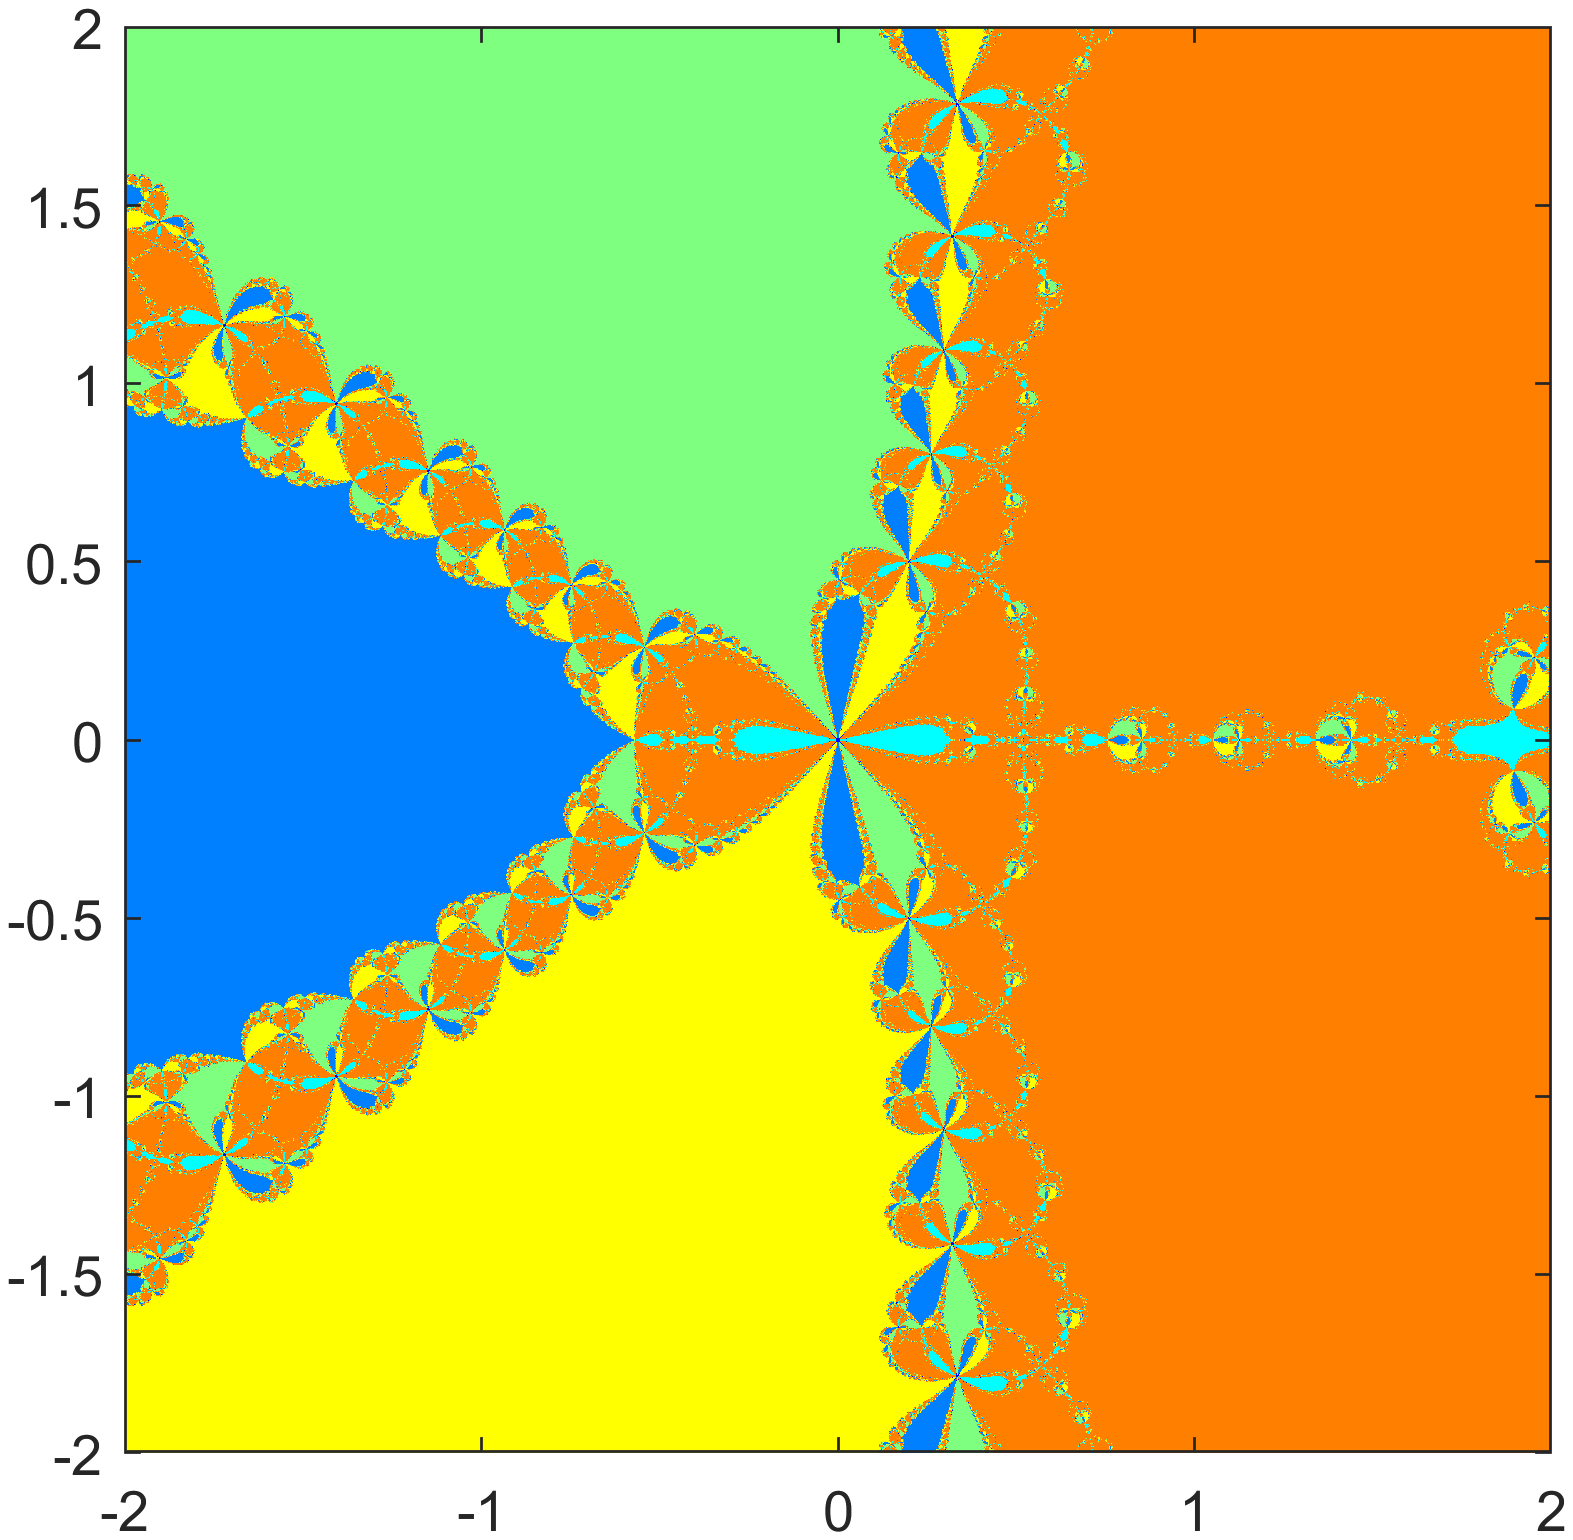
\includegraphics[width=0.6\textwidth]{figs/fractal_a.png}
    \end{minipage}
    \hfill
    \begin{minipage}[t]{0.49\textwidth}
        \vspace{0pt} % Ensure top alignment
        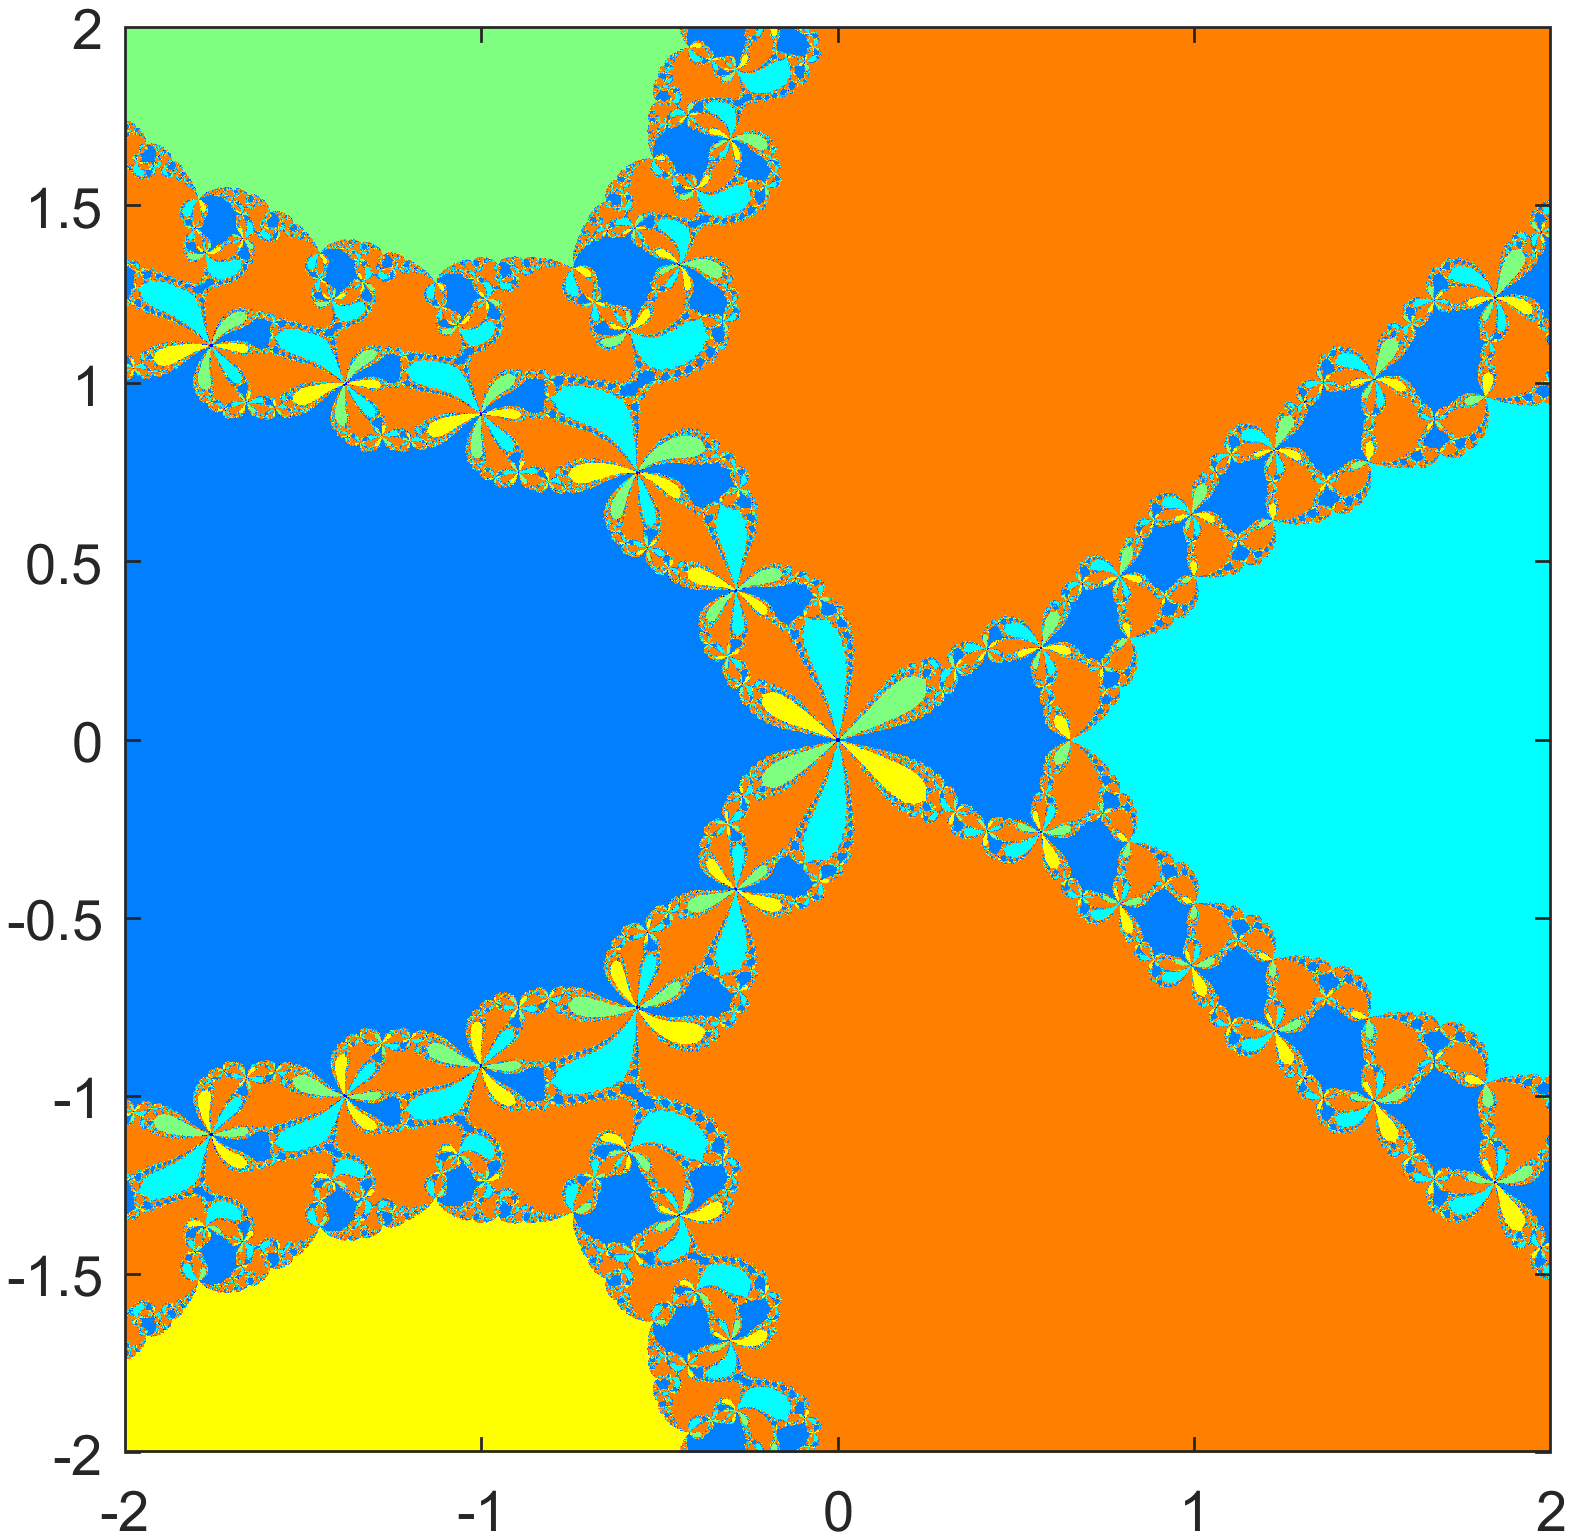
\includegraphics[width=0.6\textwidth]{figs/fractal_b.png}
    \end{minipage}
    \vskip\baselineskip % Add vertical space between rows
    \begin{minipage}[t]{0.49\textwidth}
        \vspace{0pt} % Ensure top alignment
        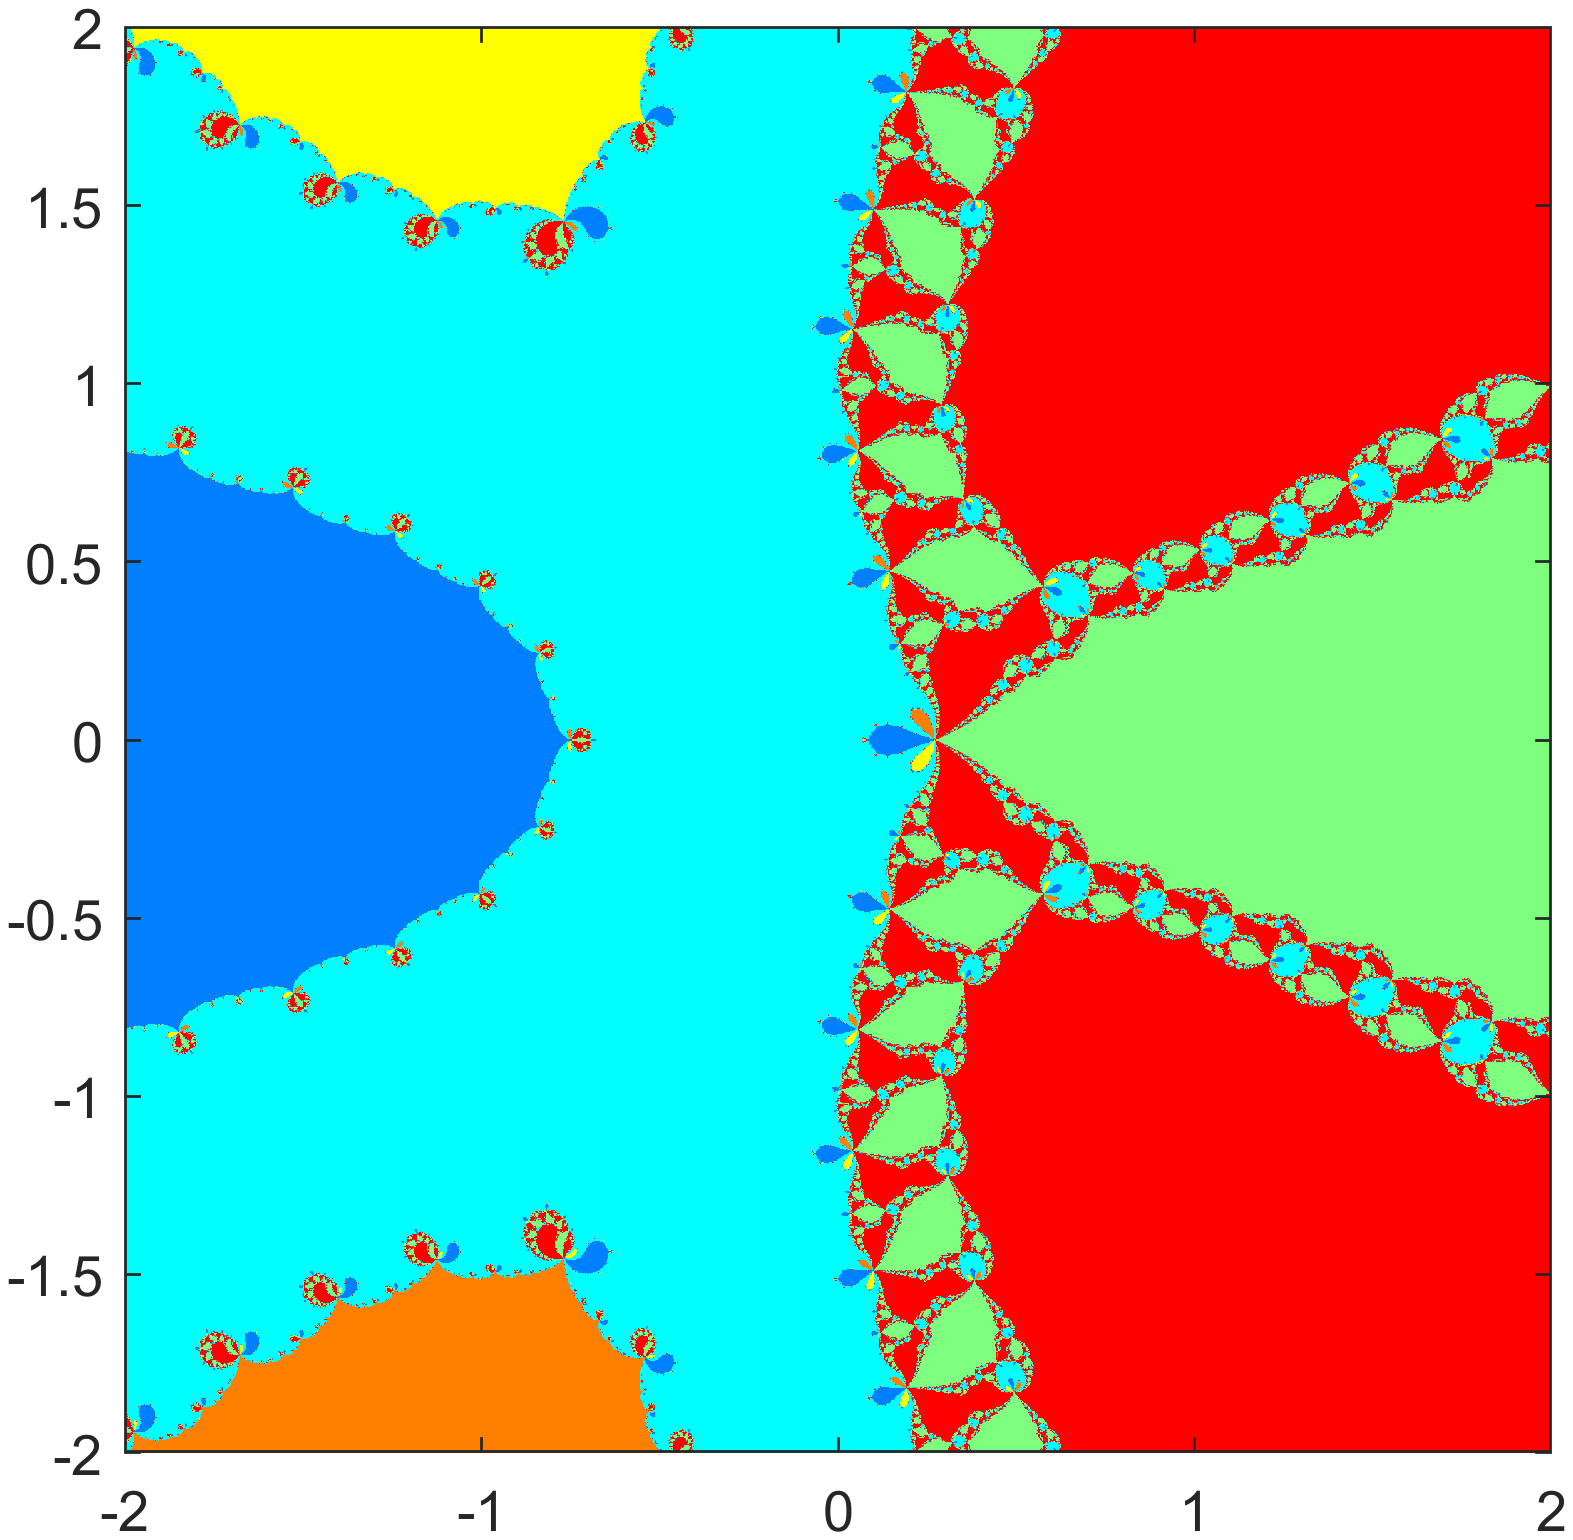
\includegraphics[width=0.6\textwidth]{figs/fractal_c.png}
    \end{minipage}
    \hfill
    \begin{minipage}[t]{0.49\textwidth}
        \vspace{0pt} % Ensure top alignment
        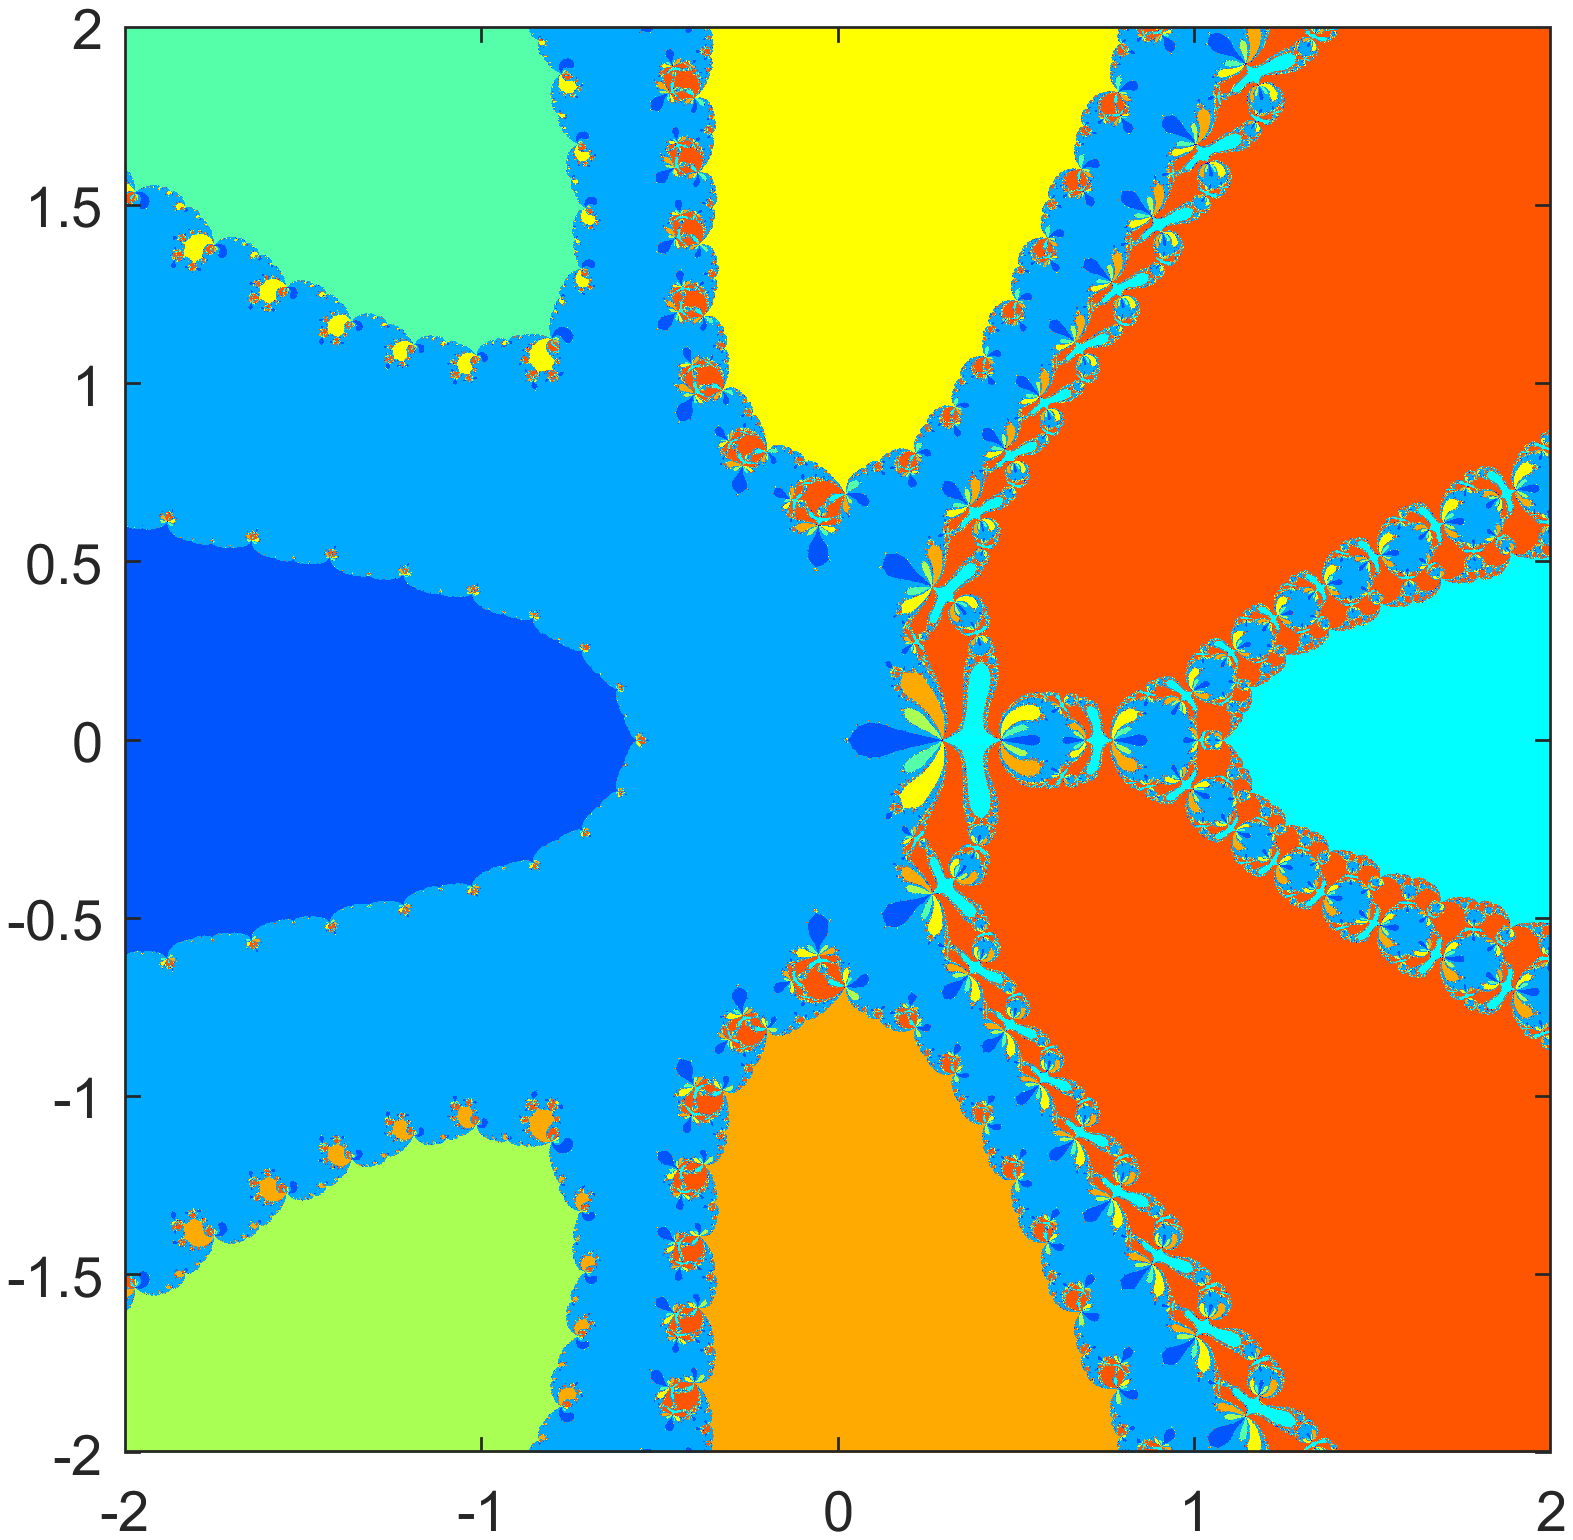
\includegraphics[width=0.6\textwidth]{figs/fractal_d.png}
    \end{minipage}
    \end{center}
\end{frame}

%%%%%%%%%%%%%%%%%%%%%%%%%
\sectionframe{Extra Topic: Higher Dimensions}
%%%%%%%%%%%%%%%%%%%%%%%%
\begin{frame}{Root-fining in higher dimensions}
    \begin{itemize}
        \item When $x$ is in 1D, root finding $f(x)=0$ is easy \\
             \raisebox{-\height}{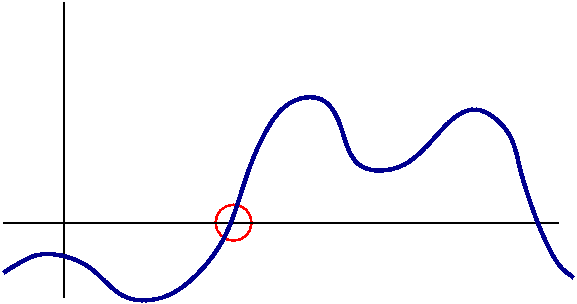
\includegraphics[scale=0.18]{figs/root.png}}
            % 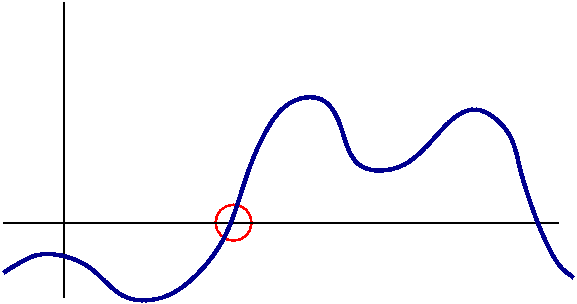
\includegraphics[scale=0.15]{figs/root.png}
        \item In 2D, solving $\textbf{F}(x,y)=0$ is harder but can be plotted\\

        \item For 3D and higher, there are no graphical tools        

        \item Solving $\textbf{f}(\textbf{x}) = \textbf{0}$ can be difficult
    \end{itemize}
\end{frame}

\begin{frame}
\frametitle{Newton's Method in Higher Dimensions}
Consider roots of $\mathbf{f}(\mathbf{x}) = \mathbf{0}$ where,
\[ \mathbf{f}(\mathbf{x}) = \begin{bmatrix}
f_1(\mathbf{x})\\
f_2(\mathbf{x})\\
\vdots \\
f_n(\mathbf{x})\\
\end{bmatrix}, \quad
\mathbf{x} = \begin{bmatrix}
x_1\\
x_2\\
\vdots \\
x_n
\end{bmatrix}, \quad \mathbf{0} = \begin{bmatrix}
0\\
0\\
\vdots\\
0
\end{bmatrix}.
\]

Example:
\[
\mathbf{f}(\mathbf{x}) = \begin{bmatrix}
\sin(x) + y  + 4\\
x^2 - xy
\end{bmatrix}
\]

Newton in one dimension:
\begin{equation*}
    x_{k+1} = x_k - \frac{f(x_k)}{f'(x_k)}
\end{equation*}

Newton  for system of nonlinear equations:
\[
\mathbf{x}_{k+1} = \mathbf{x}_{k} - [\mathbf{J}_{\mathbf{f}}(\mathbf{x}_k)]^{-1} \mathbf{f}(\mathbf{x}_k)
\]

\end{frame}

\begin{frame}
\frametitle{Newton's Method in Higher Dimensions}
\[
\mathbf{x}_{k+1} = \mathbf{x}_{k} - [\mathbf{J}_{\mathbf{f}}(\mathbf{x}_k)]^{-1} \mathbf{f}(\mathbf{x}_k)
\]
   Here $\mathbf{J}_{\mathbf{f}}$ is the Jacobian matrix (higher dimensional equivalent to a first derivative),
\[
\mathbf{J}_{\mathbf{f}}(\mathbf{x}) = \begin{bmatrix}
\frac{\partial f_1}{\partial x_1} &  \frac{\partial f_1}{\partial x_2} &  \cdots  & \frac{\partial f_1}{\partial x_n} \\
\frac{\partial f_2}{\partial x_1} &  \frac{\partial f_2}{\partial x_2} &  \cdots  & \frac{\partial f_2}{\partial x_n} \\
\vdots & \vdots& \ddots& \vdots\\
\frac{\partial f_n}{\partial x_1} &  \frac{\partial f_n}{\partial x_2} &  \cdots  & \frac{\partial f_n}{\partial x_n} \\
\end{bmatrix}
\]
Each derivative is evaluated at $\mathbf{x}_k$. \\
\vspace{3ex}

Example:
\[
\mathbf{f}(\mathbf{x}) = \begin{bmatrix}
\sin(x) + y  - 4\\
x^2 - xy
\end{bmatrix}, \qquad 
\mathbf{J}_{\mathbf{f}}(\mathbf{x}) = \begin{bmatrix}
\cos(x) & 1 \\
2x - y & -x
\end{bmatrix}
\]

Question: How do we compute  $[\mathbf{J}_{\mathbf{f}}(\mathbf{x}_k)]^{-1}$?

\end{frame}

\begin{frame}
\frametitle{Newton's Method in Higher Dimensions}
Solve (using Gaussian elimination, CG, etc...)
\[
\mathbf{J}_{\mathbf{f}}(\mathbf{x}_k) \mathbf{h}_{k} =  -\mathbf{f}(\mathbf{x}_k)
\]
and then set $\mathbf{x}_{k+1} = \mathbf{x}_{k} + \mathbf{h}_{k} $.

\vspace{3ex}

Example with initial guess $\mathbf{x}_0 = [1,-2]^T$ :
\[
\begin{bmatrix}
0.54& 1\\
4 & -1
\end{bmatrix} \mathbf{h}_0 = \begin{bmatrix}
-2.8\\
-3
\end{bmatrix}
\]

We get $\mathbf{h}_0  = [-1.2, -2.1]^T$ and so
\[
\mathbf{x}_1 = 
\begin{bmatrix}
1\\
-2
\end{bmatrix} + 
\begin{bmatrix}
-1.2\\
-2.1
\end{bmatrix}
= \begin{bmatrix}
-0.2\\
-4.1
\end{bmatrix}
\]
\end{frame}

\begin{frame}{N-dimensional Newton's Method}
For a particular $\textbf{f}(\textbf{x})$, the Jacobian $\textbf{J}_{\textbf{f}}(\textbf{x})$ is hardcoded. Then an initial guess $\textbf{x}_0$ is chosen. Let $k=0$.\\

The method:
\begin{enumerate}
    \item Compute matrix $A = \textbf{J}_{\textbf{f}}(\textbf{x}_{k})$
    \item Compute vector $\textbf{b} =  -\mathbf{f}(\mathbf{x}_k)$
    \item Solve the system $A \textbf{h}_k = \textbf{b}$
    \item Update $\textbf{x}_{k+1} = \textbf{x}_{k} + \textbf{h}_k$
    \item \texttt{k++}
    \item Repeat
\end{enumerate}


\method{Newton's Method}
{Nonlinear problem $\textbf{F}(\textbf{x})=\textbf{0}$, initial guess $\textbf{x}_0$}
{Approximate root $\textbf{x*}$}
{Generalized version of the 1D Newton's Method}
    
\end{frame}


\end{document}
